\section{Simulazione MonteCarlo e analisi dati}

Lo scopo di questa fase dell'esperimento consiste nella ricerca e messa a punto di un
metodo sperimentale di analisi degli spettri raccolti. Il lavoro si suddivide in due step:
\begin{enumerate}
 \item sviluppare un codice di simulazione MonteCarlo (MC) in ambiente ROOT nel quale si simulano molti spettri di decadimento dei muoni cosmici in un range utile di circa 3900 canali, in accordo con gli spettri acquisiti. Gli istogrammi simulati vengono quindi utilizzati per testare diversi metodi di fit per l'esrazione dei parametri fisici;
 \item utilizzare il metodo di fit stabilito nello step precedente per estrarre $\tau^+$, $\tau^-$ e $R=N^+/N^-$ dagli spettri raccolti.
\end{enumerate}
 
\subsection{Simulazione del fondo}
La prima versione del codice MC prevede la simulazione di spettri costituiti da solo rumore (che da ora in avanti chameremo anche \textit{baseline}), attraverso la generazione uniforme di numeri casuali (\lstinline{TRandom3::Uniform(double Begin,double End)}). 
I metodi testati per la stima della \textit{baseline} sono i seguenti:
\begin{itemize}
 \item media aritmetica dei contenuti dei bin dell'istogramma \lstinline{baseline};
 \item fit con il metodo del $\chi^2$ utilizzando la funzione \lstinline{pol0} (\lstinline{baseline.Fit("pol0","R")});
 \item metodo della maximum likelihood utilizzando la funzione \lstinline{pol0} (\lstinline{baseline.Fit("pol0","LR")}).
\end{itemize}

\begin{figure}[H]
 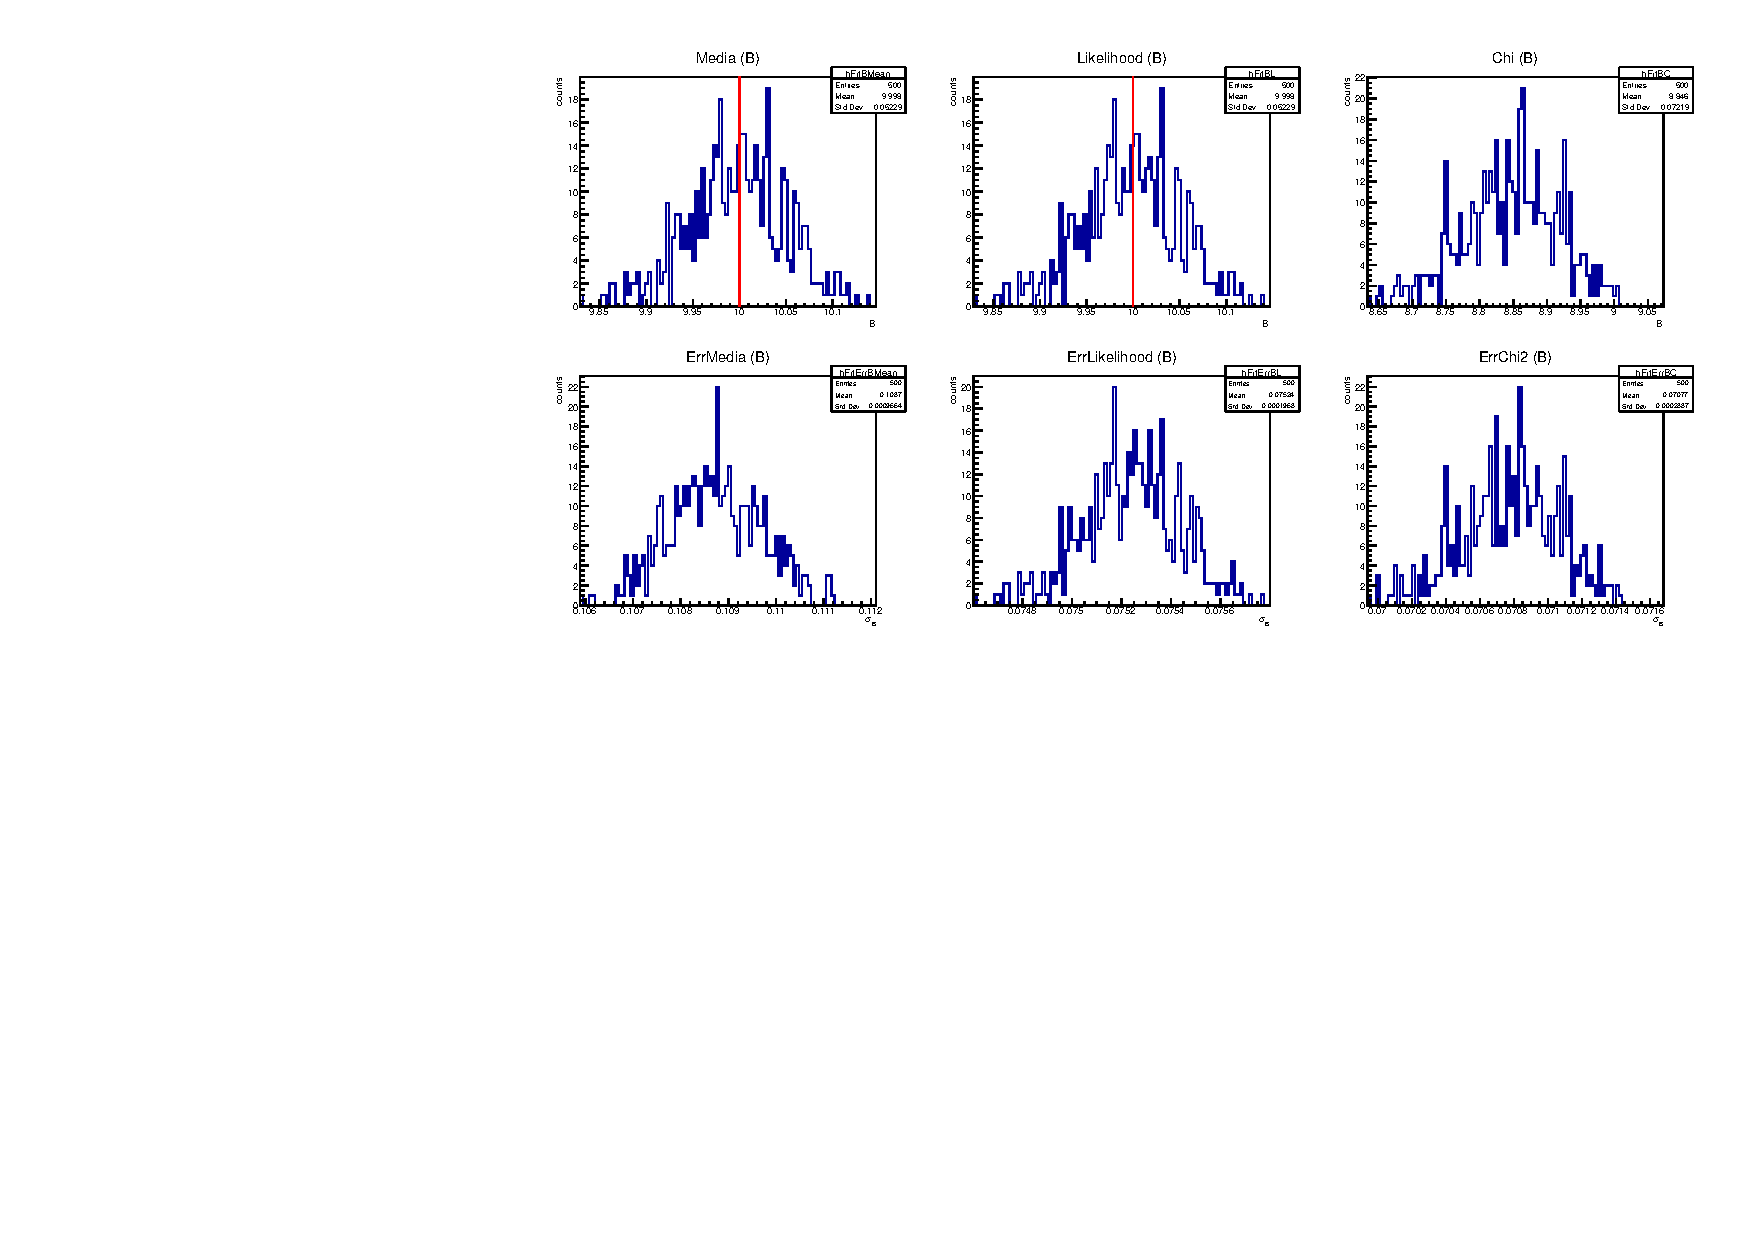
\includegraphics[scale=0.75]{img/baseline_sim_500.pdf}
 \caption{Distribuzioni delle stime della \textit{baseline} con i tre metodi differenti, sia per i valori sia per gli errori (500 simulazioni). La \textit{baseline} generata in queste simulazioni ha altezza 10.}
 \label{fig::baseline_500}
\end{figure}
In figura \ref{fig::baseline_500} è riportato un esempio delle distribuzioni dei valori e degli errori derivanti da simulazioni multiple, stimati con i tre metodi. La linea rossa verticale nei grafici in alto indica il valore vero della \textit{baseline}, ossia il valore con cui sono stati simulati gli spettri, quindi il valore che dovrebbe essere restituito dall'analisi. Come si può notare, la distribuzione dei valori estratta con fit \lstinline{pol0} di tipo $\chi^2$ non è centrata attorno al valore atteso. In questo caso, infatti, la baseline è sistematicamente sottostimata, poichè:
\begin{enumerate}
 \item il metodo dei minimi quadrati non funziona correttamente per il fit di un istogramma con bin a bassa statistica, per i quali l'assegnazione di errore di tipo poissoniano (cioè la radice del conteggio) presenta delle criticità, in particolare per contenuti nulli;
 \item il fit di una \lstinline{pol0} corrisponde esattamente ad una media pesata, nella quale i bin con statistica minore hanno un peso maggiore, con conseguenti valori sottostimati della \textit{baseline}
 \footnote{Media pesata ed errore:
 $$\bar{B}=\frac{\sum_{i=1}^N B_i/\sigma_i^2}{\sum_{i=1}^N 1/\sigma_i^2};
 \hspace{1cm} \sigma_{\bar{B}}=\frac{1}{\sum_{i=1}^N1/\sigma_i^2}
 $$}
 .
\end{enumerate}
In virtù di queste considerazioni, il metodo di fit del $\chi^2$ è stato dunque scartato. 
Gli spettri relativi agli errori statistici sulla \textit{baseline} sono utili per controllare che le distribuzioni dei valori non siano troppo disperse. In altre parole, si effettua il confronto tra la $\sigma$ delle gaussiane dei valori e il centroide $\overline{\sigma_{B}}$ delle gaussiane degli errori, controllando che $\sigma\lesssim \overline{\sigma_{B}}$, condizione soddisfatta nelle simulazioni in esame.



 